\documentclass[12pt]{article} 
\usepackage[utf8]{inputenc}
\usepackage{geometry}
\geometry{letterpaper}
\usepackage{graphicx} 
\usepackage{parskip}
\usepackage{booktabs}
\usepackage{array} 
\usepackage{paralist} 
\usepackage{verbatim}
\usepackage{subfig}
\usepackage{fancyhdr}
\usepackage{sectsty}

\pagestyle{fancy}
\renewcommand{\headrulewidth}{0pt} 
\lhead{}\chead{}\rhead{}
\lfoot{}\cfoot{\thepage}\rfoot{}

%%% SECTION TITLE APPEARANCE
\allsectionsfont{\sffamily\mdseries\upshape} 

%%% ToC (table of contents) APPEARANCE
\usepackage[nottoc,notlof,notlot]{tocbibind} 
\usepackage[titles,subfigure]{tocloft}
\renewcommand{\cftsecfont}{\rmfamily\mdseries\upshape}
\renewcommand{\cftsecpagefont}{\rmfamily\mdseries\upshape} %

\usepackage{amsmath}
\usepackage{amssymb}
\usepackage{empheq}
\usepackage{xcolor}
\renewcommand{\L}[1]{\mathcal{L}\{#1\}}
\newcommand{\ans}[1]{\boxed{\text{#1}}}
\newcommand{\vecs}[1]{\langle #1\rangle}
\renewcommand{\hat}[1]{\widehat{#1}}
\newcommand{\F}[1]{\mathcal{F}(#1)}
\title{APMA 0360: Homework 4}
\author{Milan Capoor}
\date{24 February 2023}

\begin{document}
\maketitle
\section*{Problem 1}
Solve 
\[\begin{cases}
    u_t = Du_{xx}\\
    u(x, 0) = e^{3x}
\end{cases}\]

\color{blue}
\[\F{u_t} = \F{Du_{xx}}\]
\[\frac{d}{dt}\hat{u} = (-i\kappa)^2 D \hat{u}\]
\[\frac{d}{dt}\hat{u} = -\kappa^2 D \hat{u}\]
\[\hat{u} = \F{e^{3x}}e^{-\kappa^2Dt}\]
\[\hat{u} = \F{e^{3x}}\F{\frac{1}{\sqrt{4\pi Dt}}e^{-\frac{x^2}{4Dt}}}\]
\[u(x, t) = \frac{1}{\sqrt{4\pi Dt}} \int_{-\infty}^\infty e^{3y} e^{-\frac{(x - y)^2}{4Dt}}\; dy\]
\[u(x, t) = \frac{1}{\sqrt{4\pi Dt}} \int_{-\infty}^\infty e^{3y -\frac{(x - y)^2}{4Dt}}\; dy\]
Looking at the exponent:
\begin{align*}
    3y -\frac{(x - y)^2}{4Dt} &= \frac{12Dty - (x - y)^2}{4Dt}\\
    &= \frac{12Dty - x^2 + 2xy - y^2}{4Dt}\\
    &= -\frac{y^2 - (2x - 12Dt)y + x^2}{4Dt}\\
    &= -\frac{y^2 - (2x - 12Dt)y + (x - 6Dt)^2 + x^2 - (x - 6Dt)^2}{4Dt}\\
    &= -\frac{(y - x - 6Dt)^2 + x^2 - x^2 + 12Dtx + 36D^2t^2}{4Dt}\\
    &= -\frac{(y - x - 6Dt)^2 + 12Dt(x +3Dt)}{4Dt}\\
    &= -\frac{(y-x-6Dt)^2}{4Dt} + 3(x + 3Dt)
\end{align*}
Substituting this back in, 
\begin{align*}
    u(x, t) &= \frac{1}{\sqrt{4\pi Dt}} \int_{-\infty}^\infty e^{-\frac{(y-x-6Dt)^2}{4Dt} - 3(x + 3Dt)}\; dy\\
    &= \frac{e^{3(x + 3Dt)}}{\sqrt{4\pi Dt}} \int_{-\infty}^\infty e^{-\frac{(y-x-6Dt)^2}{4Dt}}\; dy\\
    &= \frac{e^{3(x + 3Dt)}}{\sqrt{4\pi Dt}} \int_{-\infty}^\infty e^{-\left(\frac{(y-x-6Dt)}{\sqrt{4Dt}}\right)^2}\; dy\\
\end{align*}
Now u-sub with 
\[p = \frac{(y-x-6Dt)}{\sqrt{4Dt}}\]
so 
\[dp = \frac{dy}{\sqrt{4Dt}} \implies dy = \sqrt{4Dt} \; dp\]
and 
\[u(x, t) = \frac{e^{3(x + 3Dt)}}{\sqrt{4\pi Dt}} \int_{-\infty}^\infty e^{-p^2} \sqrt{4Dt} \; dp = \frac{e^{3(x + 3Dt)}}{\sqrt{\pi}} \int_{-\infty}^\infty e^{-p^2}\; dp\]
\[\boxed{u(x, t) = e^{3(x + 3Dt)}}\]

\color{black}
\pagebreak
\section*{Problem 2}
Use the Inverse Fourier Transform to solve 
\[\begin{cases}
    u_t = u_{xxxx} - 4u_{xx} + 4u\\
    u(x, 0) = f(x)
\end{cases}\]
Write your solution in terms of integrals

\color{blue}
\[\F{u_t} = \F{u_{xxxx} - 4\F{u_{xx}}} + 4\F{u}\]
\begin{align*}
    \frac{d}{dt} \hat{u} &= (-i\kappa)^4 \hat{u} - 4(-i\kappa)^2 \hat{u} + 4\hat{u}\\
    &= (\kappa^4 + 4\kappa^2 + 4)\hat{u}
\end{align*}
\begin{align*}
    \hat{u} &= \hat{f}(\kappa)e^{(\kappa^4 + 4\kappa^2 + 4)t}\\
    &= \hat{f}(\kappa)e^{(\kappa^2 + 2)^2t} 
\end{align*}
Inverse Fourier:
\[e^{(\kappa^2 + 2)^2t} = \hat{g}(\kappa, t) \Longrightarrow g(x, t) = \frac{1}{2\pi} \int_{-\infty}^{\infty} e^{(\kappa^2 + 2)^2t} e^{-i\kappa x}\; d\kappa\]
Therefore, 
\[\hat{u}(\kappa, t) = \hat{f}(\kappa) \hat{g}(\kappa, t) = \F{f \star g}(\kappa, t)\]

and 
\[\boxed{\begin{cases}
    u(x, t) = \int_{-\infty}^\infty f(y) \, g(x- y, t)\; dy\\
    \\
    \quad \text{where} \quad g(x, t) = \frac{1}{2\pi} \int_{-\infty}^{\infty} e^{(\kappa^2 + 2)^2t} e^{-i\kappa x}\; d\kappa
\end{cases}}\]
\color{black}
\pagebreak
\section*{Problem 3}
Use the inverse fourier transform to solve
\footnote{Note: Follow the steps from the Inverse Fourier Transform lecture, but this time actually evaluate the integral of the inverse
Fourier transform by completing the square with $\kappa$. You are allowed to assume that any terms at $\pm \infty$ are 0}

\[\begin{cases}
    u_t = Du_{xx}\\
    u(x, 0) = f(x)
\end{cases}\]

\color{blue}
\begin{align*}
    \F{u_t} &= D\F{u_{xx}}\\
    \frac{d}{dt} \hat{u} &= D(-i\kappa)^2 \hat{u}\\
    &= -D\kappa^2 \hat{u}\\
    \hat{u} &= \hat{f}(\kappa)e^{-D\kappa^2 t}\\
\end{align*}
\begin{align*}
    \hat{g}(\kappa, t) := e^{-D\kappa^2 t} \Longrightarrow g(x, t) &= \frac{1}{2\pi} \int_{-\infty}^{\infty} e^{-D\kappa^2 t} e^{-i\kappa x}\; d\kappa\\
    &=  \frac{1}{2\pi} \int_{-\infty}^{\infty} e^{-D\kappa^2 t -i\kappa x}\; d\kappa\\
    &= \frac{1}{2\pi} \int_{-\infty}^{\infty} e^{-Dt(\kappa^2  + \frac{ix}{Dt}\kappa)}\; d\kappa\\
    &= \frac{1}{2\pi} \int_{-\infty}^{\infty} e^{-Dt(\kappa^2 + \frac{ix}{2Dt}\kappa + \frac{x^2}{4D^2t^2} - \frac{x^2}{4D^2t^2})}\; d\kappa\\
    &=  \frac{1}{2\pi} \int_{-\infty}^{\infty} e^{-Dt(\kappa + \frac{ix}{2Dt})^2 - \frac{x^2}{4Dt}}\\
    &= \frac{1}{2\pi}e^{- \frac{x^2}{4Dt}} \int_{-\infty}^{\infty} e^{-Dt(\kappa + \frac{ix}{2Dt})^2}\; d\kappa\\
    &= \frac{1}{2\pi}e^{- \frac{x^2}{4Dt}} \int_{-\infty}^{\infty} e^{-(\kappa\sqrt{Dt} + \frac{ix}{2Dt}\sqrt{Dt})^2}\; d\kappa\\
\end{align*}
Let 
\[p =\kappa\sqrt{Dt} + \frac{ix}{2Dt}\sqrt{Dt} \implies dp = \sqrt{Dt}\; d\kappa\]
so 
\begin{align*}
    g(x, t) &= \frac{1}{2\pi}e^{- \frac{x^2}{4Dt}} \int_{-\infty}^{\infty} e^{-(\kappa + \frac{ix}{2Dt})^2}\; d\kappa\\
    &= \frac{1}{2\pi}e^{- \frac{x^2}{4Dt}} \int_{-\infty}^{\infty} e^{-p^2} \frac{1}{\sqrt{Dt}}\; dp\\
    &=  \frac{\sqrt{\pi}}{2\pi\sqrt{Dt}} e^{- \frac{x^2}{4Dt}}\\
    &= \frac{1}{\sqrt{4\pi Dt}}e^{- \frac{x^2}{4Dt}}
\end{align*}
which is just the heat kernel!

This goes all the way back to the fourier product:
\begin{align*}
    \hat{u} &= \hat{f}(\kappa) \hat{g}(\kappa, t)\\
    &= \F{(f \star g)(\kappa, t)}
\end{align*}
so 
\[\boxed{u(x, t) = \frac{1}{\sqrt{4\pi Dt}}\int_{-\infty}^\infty f(y) e^{-\frac{(x - y)^2}{4Dt}}\; dy}\]
\color{black}
\pagebreak
\section*{Problem 4}
Take the same setting as the wave equation derivation, but instead of the force being just tension, assume that the force is tension on both sides plus a resistance force $F_r$ only at (x, t) proportional to the velocity of the string but in the opposite direction. Carefully derive the resulting equation of the string and explain how you got your answer. \footnote{Hint: Most of the derivation is similar to the wave equation, and you don't need to repeat the whole thing, just tell me what modifications you have to make. You can assume that $F_r$ is some multiple of $\Delta x$}

\color{blue}
Begin with the assumptions that the string is of infinite length, thin, has uniform density $\rho$, and experiences only vertical displacement. Then,
\[F = ma = \langle0, \rho \sqrt{(\Delta x)^2 + (\Delta u)^2}\rangle u_{tt}\] 
Then, like in the tension-only wave equation derivation, we can model the string and forces acting on it with the following:

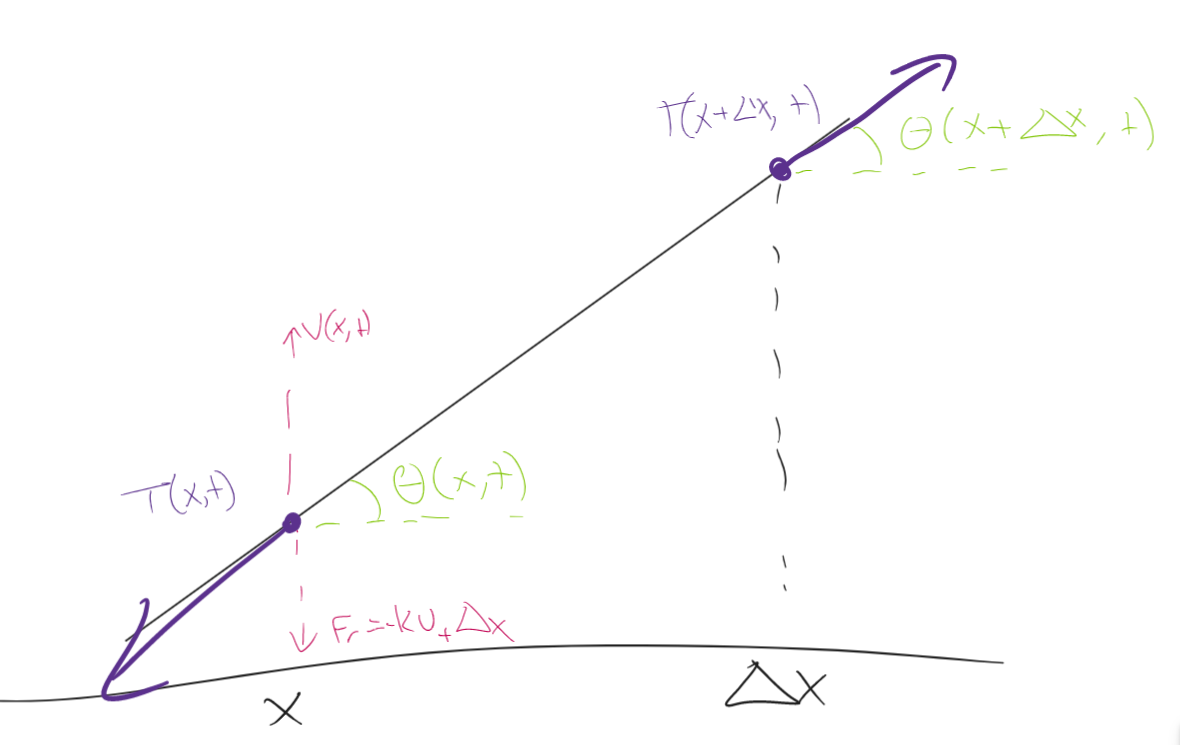
\includegraphics[width=0.8\textwidth]{Images/string force.png}

Then the force at $(x, t)$ is 
\[\langle -T\cos(\theta), -T\sin(\theta) - ku_t\Delta x\rangle(x, t)\]
for some constant k, while the force at $(x + \Delta x, t)$ is 
\[\langle T \cos(\theta), T\sin(\theta)\rangle(x + \Delta x, t)\]

The net force, therefore, is 
\[F(x, t) = \langle T \cos(\theta), T\sin(\theta)\rangle(x + \Delta x, t) + \langle -T\cos(\theta),-T\sin(\theta) - ku_t\Delta x\rangle(x, t)\]
Then using $F = ma$ and comparing the components,
\[\begin{cases}
    T(x + \Delta x, t)\cos(\theta)- T(x, t) \cos(\theta) = 0\\
    T(x + \Delta x, t)\sin(\theta) - T(x, t)\sin(\theta) - ku_t \Delta x= \rho \sqrt{(\Delta x)^2 + (\Delta u)^2} u_{tt}\\
\end{cases}\]
Rearranging, we have 
\[\begin{cases}
    T(x + \Delta x,t)\cos(\theta) - T(x, t)\cos(\theta) = 0\\
    T(x + \Delta x,t)\sin(\theta) - T(x, t)\sin(\theta) = ku_t \Delta x + \rho \sqrt{(\Delta x)^2 + (\Delta u)^2} u_{tt}(x, t)
\end{cases}\]
Dividing by $\Delta x$ and taking the limit as $\Delta x \to 0$ we get differential equations in x:
\[\begin{cases}
    \lim_{\Delta x \to 0} \frac{T(x + \Delta x,t) - T(x, t)\cos(\theta)}{\Delta x} = 0\\
    \lim_{\Delta x \to 0} \frac{T(x + \Delta x,t) - T(x, t)\sin(\theta)}{\Delta x} = \lim_{\Delta x \to 0} \frac{ku_t \Delta x + \rho \sqrt{(\Delta x)^2 + (\Delta u)^2} u_{tt}(x, t)}{\Delta x}
\end{cases}\]
\[\Longrightarrow \begin{cases}
    (T(x, t)\cos(\theta))_x = 0\\
    (T(x, t)\sin(\theta))_x = ku_t + \lim_{\Delta x \to 0} \frac{\rho \sqrt{(\Delta x)^2 + (\Delta u)^2} u_{tt}(x, t)}{\Delta x}
\end{cases}\]
Looking at the sin equation, we have 
\begin{align*}
    (T(x, t)\sin(\theta))_x &= ku_t + \lim_{\Delta x \to 0} \frac{\rho \sqrt{(\Delta x)^2 + (\Delta u)^2} u_{tt}(x, t)}{\Delta x}\\
    &= ku_t + \rho u_{tt} \sqrt{1 + (u_x)^2}
\end{align*}
But as $\Delta x \to 0$, $|u_x| << 1$, so 
\[\sqrt{1 + (u_x)^2} \approx 1\]
and 
\[(T(x, t)\sin(\theta))_x = ku_t + \rho u_{tt}\]

But if we assume the displacements $\Delta u/\Delta x$ are small, then 
\[\theta(x, t) = \tan^{-1}\frac{\Delta u}{\Delta x}\]
is also small and 
\[|\theta(x, t)| << 1 \Longrightarrow \cos(\theta) \approx 1\]

This lets us write the cos equation above as 
\[(T(x, t)\cos(\theta))_x = 0 \Longrightarrow T(x, t)_x = 0\]
so the tension does not depend on x. We now make the further assumption that tension also does not depend on time so $T(t) = T$. 

Then from trig 
\[\sin \theta = \tan \theta \cos \theta = \frac{\Delta u}{\Delta x} \cos \theta = u_x\]
so 
\[(T\sin(\theta))_x = (Tu_x)_x = ku_t + \rho u_{tt}\]
Then because T is constant,
\[(Tu_x)_x = Tu_{xx} = ku_t + \rho u_{tt}\]
So at last we have, 
\[u_{tt} = \frac{T}{\rho}u_{xx} - \frac{k}{\rho}u_t\]
let $c = \sqrt{T/\rho}$ as usual and $\kappa = k / \rho$ 
\[\boxed{u_{tt} = c^2 u_{xx} + \kappa u_t}\]

\color{black}
\pagebreak
\section*{Problem 5}
Use the Fourier transform to find the general
solution of the wave equation
\[u_{tt} = c^2 u_{xx}\]
Write your answer explicitly, without integrals \footnote{Hint: use the fact that 
\[y'' + a^2y = 0 \implies y(t) = Ae^{iat} + Be^{-iat}\] 
and the shifting property 
\[e^{ika} \hat{f}(\kappa) = \hat{g}(\kappa) \quad g(x) = f(x - a)\]}
\color{blue}
\[\F{u_{tt}} = c^2\F{u_{xx}}\]
\[\frac{d^2}{dt^2}\hat{u} = c^2 (-i\kappa)^2 \hat{u}\]
\[\frac{d^2}{dt^2}\hat{u} + c^2\kappa^2 \hat{u} = 0 \Longrightarrow  \hat{u}(\kappa, t) = \hat{A}(\kappa)e^{ic\kappa t} + \hat{B}(\kappa)e^{-ic\kappa t}\]
\begin{align*}
    u(x, t) &= \frac{1}{2\pi} \int_{-\infty}^\infty \hat{A}(\kappa) e^{i\kappa x}e^{ic\kappa t}\; d\kappa + \frac{1}{2\pi} \int_{-\infty}^\infty \hat{B}(\kappa) e^{i\kappa x}e^{-ic\kappa t}\; d\kappa\\
    &= \frac{1}{2\pi} \int_{-\infty}^\infty \hat{A}(\kappa) e^{(x + ct)i\kappa}\; d\kappa + \frac{1}{2\pi} \int_{-\infty}^\infty \hat{B}(\kappa) e^{(x- ct)i\kappa}\; d\kappa\\
    &= \frac{1}{2\pi} \int_{-\infty}^\infty \F{A(x - ct)} \; d\kappa + \frac{1}{2\pi} \int_{-\infty}^\infty \F{B(x + ct)} \; d\kappa\\
    &=\boxed{A(x-ct) + B(x + ct)}
\end{align*}
\end{document}